\documentclass[class=book, crop=false, oneside, 12pt]{standalone}
\usepackage{standalone}
\usepackage{amsmath}
\usepackage{../../style}
\graphicspath{{./assets/images/}}

% arara: pdflatex: { synctex: yes, shell: yes }
% arara: latexmk: { clean: partial }
\begin{document}

\chapter{Campo magnetico, forza magnetica}

\section{Interazione magnetica, campo magnetico}

La proprietà di attirare la limatura di ferro, mostrata da alcuni minerali di ferro e in particolare dalla \emph{magnetite}, era già nota nel passato, il fenomeno prese il nome di magnetismo.
Tale proprietà di attrazione non è uniformemente presente nel materiale, ma si manifesta principalmente in determinate parti, ed è in particolare possibile costruire campioni cilindrici in cui essa è localizzata nella zona delle basi. 
Sia questi oggetti che altri con diversa geometria si indicano col nome di \emph{magneti} e le parti in cui si localizza la proprietà di attrazione si chiamano i poli del magnete.

Gilbert compì una serie di esperienze con magneti, aventi lo scopo di mettere in evidenza le caratteristiche del magnetismo e le differenze con i fenomeni di elettrostatica, da lui stesso studiati. 
I risultati sullo studio delle interazioni tra poli magnetici, anche tenendo conto di successive osservazioni, sono riassunti nei punti seguenti.

\begin{enumerate}
    \item Se ad un magnete sospeso nel centro tramite un filo, e quindi libero di ruotare, si avvicina un secondo magnete, tenuto ad esempio in mano, si osserva che questo esercita sul primo una certa forza. 
    Come per le forze di natura elettrostatica, possiamo interpretare il fatto dicendo che un magnete genera un campo, chiamato \emph{campo magnetico}, e che l'altro magnete risente dell'azione che il campo magnetico esercita nella posizione da esso occupata. 
    Un'analisi sistematica porta a stabilire che la forza di interazione tra i due magneti è attrattiva o repulsiva a seconda dei poli dei magneti che vengono affacciati e che esistono soltanto due specie di \emph{poli}, detti \emph{poli positivi} e \emph{poli negativi}; inoltre si trova che \emph{i poli di uno stesso magnete sono sempre di segno opposto}. 
    \begin{figure}[h]
        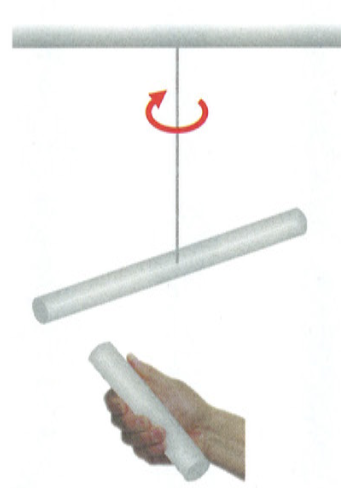
\includegraphics[scale=0.4]{magnete_filo.png}
        \centering
        \caption{}
    \end{figure}
    \item Se si avvicina a un pezzo di magnetite una bacchetta sottile di ferro, questa acquista la proprietà di attirare la limatura di ferro, principalmente in vicinanza delle estremità: la bacchetta di ferro immersa nel campo magnetico generato dalla magnetite è diventata pertanto un magnete, ovvero si è magnetizzata. 
    Essa viene chiamata magnete artificiale o calamita e presenta due poli magnetici di segno opposto. 
    Soprattutto se è di piccole dimensioni la bacchetta viene anche detta ago magnetico. 
    \item Se sospendiamo ad un filo l'ago magnetico sopra definito e lo lasciamo libero di ruotare, osserviamo che esso tende a disporsi approssimativamente parallelo al meridiano terrestre; spostato da questa posizione di equilibrio l'ago compie intorno ad essa oscillazioni, smorzate inevitabilmente dagli attriti. 
    L'esperienza mostra l'esistenza di un campo magnetico naturale,\emph{il campo magnetico terrestre}, e mette in evidenza un comportamento dell'ago magnetico del tutto analogo a quello di un dipolo elettrico posto in un campo elettrico \(\overrightarrow{E}\). 
    L'ago magnetico, in altre parole, si comporta come un \emph{dipolo magnetico} che lasciato libero si orienta nella direzione e verso del campo magnetico esistente nel punto dove è posto. 
    Il polo dell'ago che si orienta approssimativamente verso il nord geografico, viene chiamato \emph{polo nord} (N) e  gli si attribuisce segno \emph{positivo}, l'altro è chiamato \emph{polo sud} (S) e  gli si dà segno \emph{negativo}. 
    Definiti nel modo detto i poli di un magnete ed eseguendo esperienze come quelle del punto A, si trova sempre che l'interazione tra \emph{poli magnetici dello stesso segno è repulsiva}, quella tra \emph{poli magnetici di segno opposto attrattiva}.
    \item Lo studio quantitativo della forza magnetica tra i poli di due magneti, svolto da Coulomb, dimostrò anche in tale caso un andamento inversamente proporzionale al quadrato della distanza, almeno per poli puntiformi, come sono con buona approssimazione quelli agli estremi di sbarre lunghe e sottili. 
    Sebbene la forza che si esercita tra due poli magnetici sia simile a quella che si esercita tra due cariche elettriche, esiste tra di esse una differenza fondamentale. 
    Una carica elettrica, positiva o negativa, può sempre essere isolata e ciò è una conseguenza dell'esistenza della carica elementare positiva portata dal protone e della carica elementare negativa portata dall'elettrone: la possibilità di separazione esiste cioè già a livello elementare. 
    Invece non è mai stato possibile ottenere un polo magnetico isolato: i poli magnetici sembrano esistere sempre a coppie di egual valore e segno opposto, cioè si manifestano solamente sotto forma di dipoli magnetici. 
    L'indicazione classica è costituita dall'esperimento della calamita spezzata. 
    Se si taglia a metà una calamita compaiono sempre due poli di segno opposto nella zona del taglio, che precedentemente a questo non mostrava la proprietà di attirare limatura di ferro. 
    Ripetendo il taglio su pezzi sempre più piccoli si ottiene ogni volta lo stesso risultato, senza riuscire ad ottenere un polo magnetico isolato (monopolo magnetico). 
    \begin{figure}[h]
        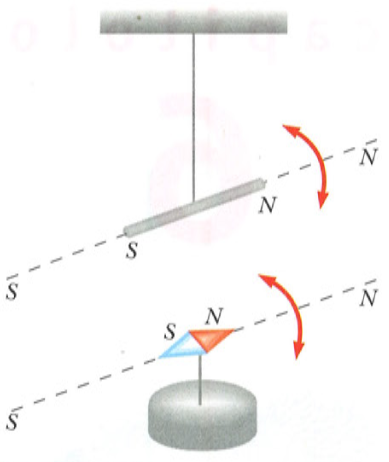
\includegraphics[scale=0.4]{orientamento_dipoli_magnetici.png}
        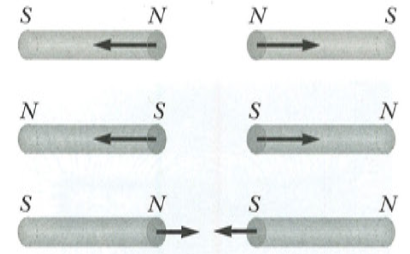
\includegraphics[scale=0.4]{forze_poli.png}
        \centering
        \caption{}
    \end{figure}
    \item Accanto a tale esperienza sono significative quelle condotte con limatura di ferro posta in vicinanza di un magnete. 
    I granelli di limatura si dispongono in modo ordinato lungo linee regolari, fatto che interpretiamo supponendo che ciascun granello venga magnetizzato dal campo magnetico del magnete e diventato un dipolo magnetico si orienti parallelamente al campo magnetico stesso.
\end{enumerate}
In analogia a quanto fatto per il campo elettrico \(\overrightarrow{E}\), possiamo definire le linee di campo magnetico, cioè quelle linee che in ogni punto sono tangenti al campo magnetico esistente in quel punto. 
Tale vettore viene indicato con il simbolo \(\overrightarrow{B}\). 
Il verso delle linee di \(\overrightarrow{B}\) può essere individuato ponendo un piccolo ago magnetico in ciascun punto in cui esiste il campo \(\overrightarrow{B}\). 
Esso infatti si orienterà parallelamente a \(\overrightarrow{B}\) e il verso sarà quello che va dal polo Sud al polo Nord dell'ago magnetico. 
Valgono per il campo magnetico \(\overrightarrow{B}\) le proprietà a, b, e, per le linee di forza del campo elettrostatico \(\overrightarrow{E}\) e inoltre pure la proprietà che un campo magnetico \(\overrightarrow{B}\) uniforme sia rappresentato da linee parallele ed equidistanti. 

\section{Elettricità e magnetismo}

\begin{figure}[h]
    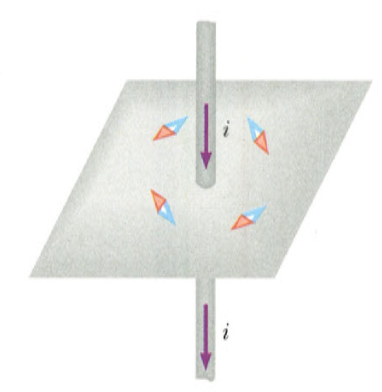
\includegraphics[scale=0.4]{corrente_campo.png}
    \centering
    \caption{}
\end{figure}

La prima relazione tra fenomeni magnetici ed elettrici fu scoperta da Oersted.
Oersted mostrò che un ago magnetico, posto in prossimità di un filo percorso da corrente, tende ad assumere una ben definita posizione di equilibrio. 
Se poniamo in un piano perpendicolare al filo percorso da corrente della limatura di ferro, osserviamo che i grani si addensano lungo circonferenze con centro il filo. 
Alla luce di quanto visto finora il risultato si interpreta dicendo che il filo percorso da corrente produce un campo magnetico \(\overrightarrow{B}\) e che l'ago e i grani di limatura di ferro si orientano parallelamente al campo magnetico esistente nel punto in cui sono posti. 
\begin{figure}[h]
    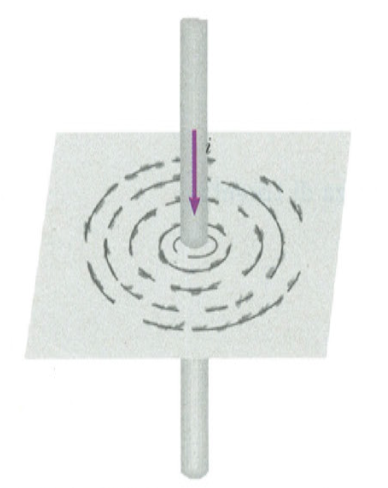
\includegraphics[scale=0.4]{campo_magnetico_filo_corrente.png}
    \centering
    \caption{}
\end{figure}
In seguito Ampère dimostrò che anche due fili percorsi da corrente interagiscono e intuì che le azioni magnetiche non sono altro che la manifestazione dell'interazione tra cariche elettriche in movimento, ponendo le basi della teoria attuale del magnetismo. 
In particolare due fili in cui è percorsa una corrente nella stessa direzione si attraggono, se la corrente è percorsa in direzione opposta si respingono.

\begin{figure}[h]
    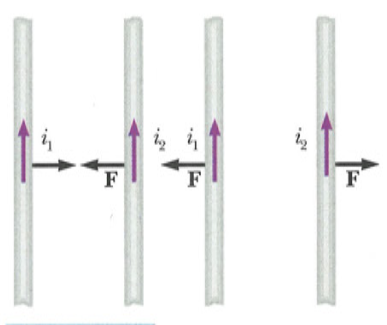
\includegraphics[scale=0.4]{int_cavi.png}
    \centering
    \caption{}
\end{figure}

\section{Legge di Gauss per il campo magnetico}

Dato che ogni carica magnetica positiva è accompagnata da una carica magnetica negativa, non posso avere una superficie con mezza carica di prova.
Quindi la somma delle cariche magnetiche è sempre \(0\).

Il teorema di Gauss per il campo magnetico mi dice quindi 
\begin{equation}
    \Phi \left(\overrightarrow{B}\right) = \oint_{\Sigma} \overrightarrow{B} \cdot \overrightarrow{u}_x d \Sigma = 0
\end{equation}
Per questo dico che il campo magnetico è \emph{solenoidale}.
Infatti, a differenza delle linee di campo di una carica elettrica che vanno a infinito, le linee di campo di un campo magnetico sono sempre chiuse.

\end{document}